\documentclass[12pt,twoside,book]{article}

\input{../settings}

\begin{document}

%%%%%%%%%%%%%%%%%%%%%%%%%%%%%%%%%%%%%%%%%%%%%%%%%%%%%%%%%%%%%%%%%%%%%%%%%%%%%%%
\section{Structure of the loop functions}
\label{sec:reim}
%%%%%%%%%%%%%%%%%%%%%%%%%%%%%%%%%%%%%%%%%%%%%%%%%%%%%%%%%%%%%%%%%%%%%%%%%%%%%%%

\vskip 0.1in

In this section, we examine the structure of the loop functions defined in Sec.~\ref{sec:dy} and discuss their properties.
Recall the form of the loop functions
\begin{align}
  f(x) = \begin{cases}
    \displaystyle{\frac{1}{16\pi^2} \int_0^1 dy\, (1-2y)^2 \ln (1-
    y(1-y)x - i0)} & {\rm (Scalar)},\\[5mm]
	  %%
    \displaystyle{\frac{1}{16\pi^2} \int_0^1 dy\, y(1-y) \ln (1 -
	  y(1-y)x - i0)} & {\rm (Fermion)},
  \end{cases}\label{app_eq_f}
\end{align}
which correspond to the vacuum polarization effects from scalar and fermionic WIMPs, respectively.
Note that $f(x=0) = 0$ for both scalar and fermionic cases.

First, we consider the imaginary part of Eq.~\eqref{app_eq_f}.
The imaginary part of the integrand is non-zero if and only if $1-y(1-y) x < 0$, which can be realized when $x > 4$.
Under this condition, we can evaluate the integral and obtain
\begin{align}
  \Im f(x) = \begin{cases}
    \displaystyle{-\frac{1}{48\pi} \beta^3} & (\text{Scalar}, \,x>4),\\
    \displaystyle{-\frac{1}{192\pi} \beta (3 - \beta^2)} & (\text{Fermion}, \,x>4),
  \end{cases}
  \label{eq:imf}
\end{align}
with $\beta \equiv \sqrt{1-4/x}$.
According to the optical theorem, $\Im f(x)$ is proportional to the parton-level WIMP pair production cross section discussed in Sec.~\ref{sec:wimp_production} with a negative coefficient, and thus $\Im f(x) < 0$ for any $x>4$.
Note that, if we substitute $x = s'/m_\chi^2$, the $\beta$ dependence of Eq.~\eqref{eq:imf} is consistent with the total pair production cross section that is obtained by integrating Eqs.~\eqref{eq:parton_cross_section_scalar} and \eqref{eq:parton_cross_section_fermion} over the solid angle.
In the pair production process, $\beta$ denotes the velocity of the produced WIMPs in the CM frame.

\begin{figure}[t]
  \centering
  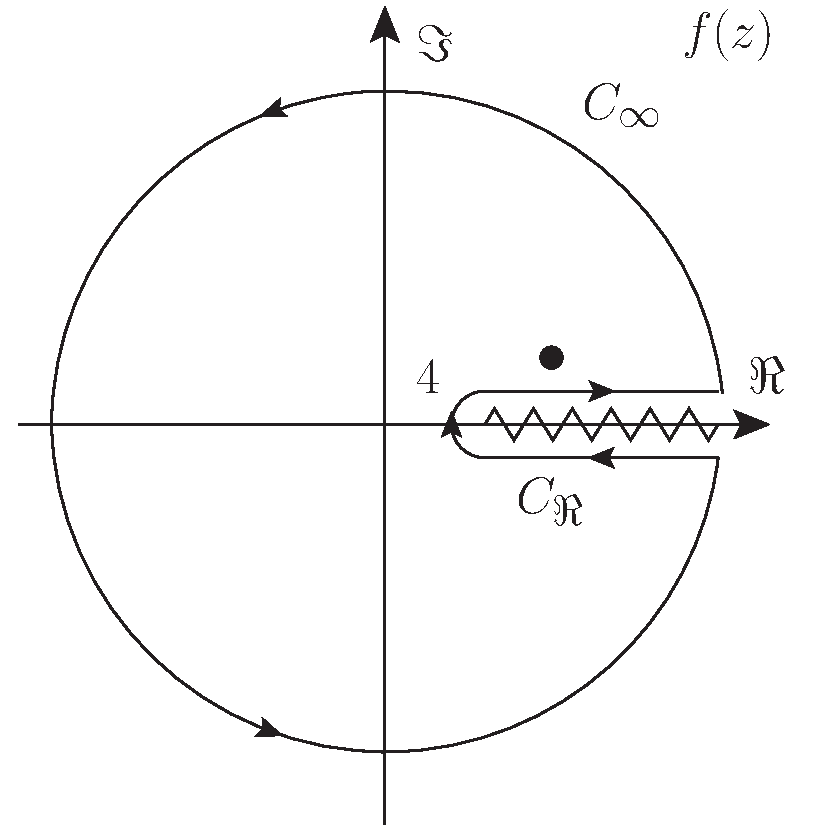
\includegraphics[width=0.5\hsize]{Analytic-loop-function.pdf}
  \caption{Analytic structure of the loop function $f(z)$ and the contour of the integration.}
  \label{fig:analytic}
\end{figure}

Next, we consider the analytic structure of the loop function $f(z)$ now defined for $z \in \mathbb{C}$.
As shown in Fig.~\ref{fig:analytic}, $f(z)$ has a branch cut on the real axis with $\Re z > 4$.
Note that, in the following discussion, we take account of the Feynman prescription $-i 0$ in the loop function by choosing physically interesting points as $z = x + i0$ with $x > 0$ as shown by the black circle, while keeping the position of the branch cut just on the real axis.
From the Cauchy's theorem, we have an identity
\begin{align}
  f(z) = \frac{z}{2\pi i} \oint \frac{f(z')}{z' (z' - z)} dz',
\end{align}
where a contour that surrounds the point $z$ is chosen.
The factor $z/z'$ is introduced to realize the required property $f(z=0) = 0$.
We can take a contour shown in Fig.~\ref{fig:analytic}, which is decomposed into two parts; $C_\infty$, which exists at $|z'| \to \infty$, and $C_{\Re}$, which exists just below and above the real axis with $\Re z' > 4$.
Since the integrand decreases as $\ln z' / z^{'2}$ as $|z'|$ increases, the integration along the contour $C_\infty$ gives zero.
On the other hand, the integration along $C_\Re$ is equivalent to the integration of $f(z) - f(z)^{*} = 2i \Im f(z)$ for an analytic function $f(z)$ and we obtain
\begin{align}
  f(z) = \frac{z}{\pi} \int_4^\infty dz' \frac{1}{z' (z'-z)} \Im f(z).
  \label{eq:ffromimf}
\end{align}

From Eq.~\eqref{eq:ffromimf}, we determine the property of $\Re f$ that is important for the discussion in Sec.~\ref{sec:dy}.
For this purpose, we return to the function $f(x)$ of real values and rewrite Eq.~\eqref{eq:ffromimf} as
\begin{align}
  f(x) = \begin{cases}
    \displaystyle{\frac{x}{\pi} \int_4^\infty dx' \frac{1}{x' (x'-x)} \Im f(x)}, & (x < 4)\\
    \displaystyle{\frac{x}{\pi}\, \mathrm{P} \int_4^\infty dx' \frac{1}{x' (x'-x)} \Im f(x) + i \Im f(x)}, & (x > 4)
  \end{cases}
\end{align}
where the symbol $\mathrm{P}$ deontes the Cauchy principal value.
Note that the first term of the second line shows the real part of $f(x)$, while the second term is consistently derived by calculating the residue at $x' \to x$.
For $x<4$, we can see that $\Re f(x) = f(x) < 0$ since the integrand is always negative.
For $x>4$, the integration contains both the negative and positive contributions but we expect $\Re f(x) < 0$ for $x \sim 4$ from the continuity.
This explains the behavior of the correction to the cross section from WIMPs shown in Fig.~\ref{fig_sqsp_vs_del}.

\end{document}
